\documentclass[12pt]{article}
\usepackage[utf8]{inputenc}

\usepackage[margin = 0.7in]{geometry}
\usepackage{amsmath}
\usepackage{amsfonts}
\usepackage{amssymb}
\usepackage{amsthm}
\usepackage{graphicx}
\usepackage{placeins}
\usepackage{enumitem}
\usepackage{dsfont}

\newcommand{\N}{\mathbb{N}}
\newcommand{\Z}{\mathbb{Z}}
\newcommand{\R}{\mathbb{R}}
\newcommand{\E}{\mathbb{E}}
\newcommand{\Q}{\mathbb{Q}}
\newcommand{\de}{\mathrm{d}}
\newcommand{\one}{\mathds{1}}

\title{ECON 899: Problem Set 2}
\author{Katherine Kwok\footnote{I collaborated with Anya Tarascina and Claire Kim on this assignment.}}
\date{September 2021}

\begin{document}

\maketitle
\noindent \textbf{Overview: } For this assignment, the goal is to replicate the analysis in Huggett (1993), and compare the differences in welfare between complete and incomplete markets.\\\\
% Part 1
\noindent \textbf{Section I - Huggett with Complete Markets: } \\\\
In this section, we look at the competitive equilibrium allocations and prices under a modified version of Huggett (1993). In particular, we assume that ``there are enforceable insurance markets regarding the idiosyncratic shocks to earnings and there are no initial asset holdings" (from Problem Set 2 handout).\\\\
Assuming complete markets and locally non-satiated preferences, we know that the first and second welfare theorems hold. So, we can solve the social planner's problem, and then decentralize by finding the asset prices that would enable the social planner's allocations. The social planner's problem is: 
\begin{align*}
    &\max_{\{c_t^e, c_t^u\}_{t=0}^{\infty}} \sum_{t=0}^{\infty} \beta^t (p \cdot U(c^e_t) + (1-p) \cdot U(c_t^u)) \\
    &\text{s.t. } pc_t^e + (1-p)c_t^u = py(e) + (1-p) y(u), \forall t
\end{align*}
where $p$ is the fraction of the population that is employed and $(1-p)$ is the fraction of the population that is unemployed (i.e. invariant distribution). And $y(e)$ and $y(u)$ are the incomes of employed and unemployed individuals, respectively. Then, we can take the first order conditions to solve for the social planner's allocation: 
\begin{align*}
    \text{(w.r.t. $c_e^t$) } & p U'(c_t^e) + \lambda_t p = 0\\
    &\implies U'(c_t^e) = -\lambda_t \\
    \text{(w.r.t. $c_u^t$) } & (1-p) U'(c_t^u) + \lambda_t (1-p) = 0 \\
    &\implies U'(c_t^u) = -\lambda_t \\
\end{align*}
Therefore, $U'(c_t^e) = U'(c_t^u)$ implies that $c_t^e = c_t^u = py(e) + (1-p)y(u)$. Given $y(e) = 1$ and $y(u) = 0.5$, $c_t^e = c_t^u = p + 0.5y(u)$. \\\\
Note that employed and unemployed individuals consume equal amounts. Now, we decentralize the problem, assuming that households face price $q_t$ and choose $a_{t+1}^e$, $a_{t+1}^u$, and $H_t$ (labor) given their constraints. Here, we assume everyone who is employed works the same amount so $H_t=1$. Then,  each individual's utility maximization problem becomes:
\begin{align*}
    \max_{\{c_t^i\}_{t=0}^{\infty}} \sum_{t=0}^{\infty} &E_0 \beta^t U(c^i_t) \\
    \text{s.t. } c^i_t + q_t a^i_{t+1} &= a^i_t + y(i)
\end{align*}
where $i$ is the employment state. Then, we can plug in the budget constraint and take the first order condition with respect to $a^i_{t+1}$:
\begin{align*}
    0 &= q_t \beta^t U'(c^i_t) - \beta^{t+1} U'(c^i_{t+1}) \\
    q_t &= \frac{\beta^{t+1} U'(c^i_{t+1})}{\beta^t U'(c^i_t)} \\
    q_t &= \beta 
\end{align*}

% Part 2
\pagebreak
\noindent \textbf{Part II - Computing Huggett with Incomplete Markets: } \\\\
Next, we compute Huggett in an incomplete markets environment. The algorithm is as follows: For a given bond price $q \in [0, 1]$, we solve the value function iteration (T operator) to find an employed and unemployed individuals' policy functions ($a' = g(a, s;q)$). Then, we solve for the invariant wealth distribution $\mu(A, S;q)$ using the $T^*$ operator, which tells us conditional on a person making the decision $a' = g(a, s;q)$ today, where they fall in the wealth distribution tomorrow. Finally, we check if the given bond price $q$ generates a net asset supply (using the policy function and invariant wealth distribution) that satisfies the market clearing condition. For example, if net asset supply is positive and above the tolerance threshold, it means individuals are saving too much so the bond price should be raised so interest rate falls. \\\\
Given the model and parameters provided in the handout, we have the following results: Below, we plot the policy functions for employed and unemployed individuals. 

\begin{figure}[!htbp]
    \centering
    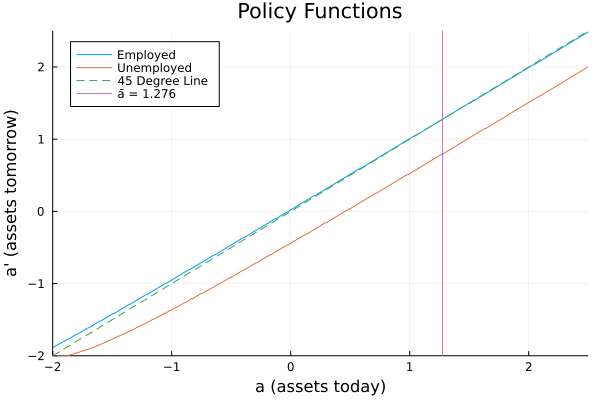
\includegraphics[width = 0.7\textwidth]{Policy_Functions.png}
    \caption{Policy Function}
    \label{fig:pol}
\end{figure}

\noindent Similar to Huggett's results, we see that the decision rule is lower for those unemployed in comparison to those who are employed. Also, we see that the decision rule for employed agents intersects with the 45 degree line, which is the $\bar{a} = 1.276$ point where $\bar{a} > g(\bar{a}, s)$. This characteristic of the decision rule establishes an upper bound so that we can solve for the invariant distribution. \\\\
\clearpage
The equilibrium bond price is 0.9942. This satisfies the constraint that $\beta < q < 1$, where $\beta = 0.9932$ for this computational exercise. Below, we see a similar steady state wealth distribution as in Huggett (1993). In particular, we see a spike slightly above $wealth = 2$, because of the upper bound $\bar{a}$ where employed individuals will stay at. Another observation to note is, there some some larger spikes on the left end for unemployed agents, indicating that those unemployed are more likely to have debt. 

\begin{figure}[!htbp]
    \centering
    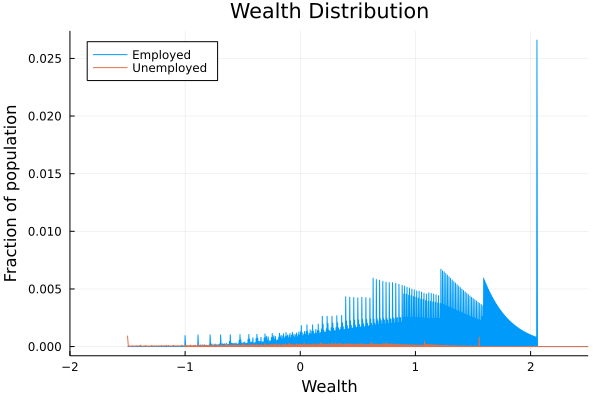
\includegraphics[width = 0.65\textwidth]{Wealth_Distribution.png}
    \label{fig:wealth}
\end{figure}

\noindent Another way to think about wealth distribution is to plot the Lorenz curve, which is below. The 45 degree line embodies a world where is not inequality in wealth distribution at all. The lorenz curve plots the fraction of agents against the fraction of wealth they hold. The associated Gini coefficient is 0.4013. This is quite close to the current Gini coefficient for the U.S., which is around 0.41 as of 2021.\footnote{https://data.worldbank.org/indicator/SI.POV.GINI?locations=US}

\begin{figure}[!htbp]
    \centering
    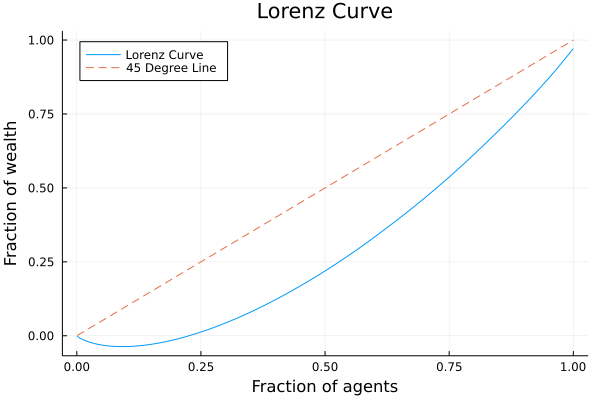
\includegraphics[width = 0.65\textwidth]{Lorenz_Curve.png}
    \label{fig:lorenz}
\end{figure}

\clearpage
% Part 3
\noindent \textbf{Part III - Welfare Analysis: } \\\\
\textbf{Complete Markets Welfare: }Finally, we want to compare the welfare of agents in complete versus incomplete financial markets. To do so, we want to first compute the wealth value in the first best allocation (complete markets). Recall that in Part I, we found that employed and unemployed individuals would consume the same amount in complete markets. Then, we only need to compute the invariant distribution of employed and unemployed individuals by iterating the Markov transition matrix a large number of times (multiply the matrix by itself), which gives the fractions $p_e = 0.9434$ and $p_u = 1 - p_e = 0.0566$. Then, the welfare in first best allocation is 
\begin{align*}
    W_{FB} &= \sum_{t=0}^{\infty} \beta^t \frac{(c_t^{FB})^{1-\alpha}}{1-\alpha} = \frac{(c_t^{FB})^{1-\alpha}}{(1-\beta)(1-\alpha)} \\
    \text{where } c_t^{FB} &= y(e) \cdot 0.9434 + y(u) \cdot 0.0566 = 0.9434 + 0.5 \cdot 0.056
\end{align*}
Given the parameter values $\alpha = 1.5$ and $\beta = 0.9932$, I estimate $W_{FB} = -4.2525$. This is slightly more positive than Dean's estimate of -4.8192. \\\\
\textbf{Consumption Equivalence: }Next, we compute the consumption equivalence $\lambda(a, s)$. Intuitively, it is the amount of consumption an agent in an incomplete market is willing to forgo in order to reach their consumption allocation in a complete market. Given the definitions of $W_FB$ and $\lambda$, we can compute $\lambda(a, s)$ by 
\begin{align*}
    \lambda(a, s) = \Bigg[\frac{W_{FB} + \frac{1}{(1-\alpha)(1-\beta)}}{v(a, s) + \frac{1}{(1-\alpha)(1-\beta)}} \Bigg]
\end{align*}
The estimated $\lambda(a, s)$ for our computational exercise is shown below, separately for employed and unemployed agents. As expected, individuals who are unemployed are willing to pay more in terms of consumption to reach their complete market allocation, compared to employed individuals.
\begin{figure}[!htbp]
    \centering
    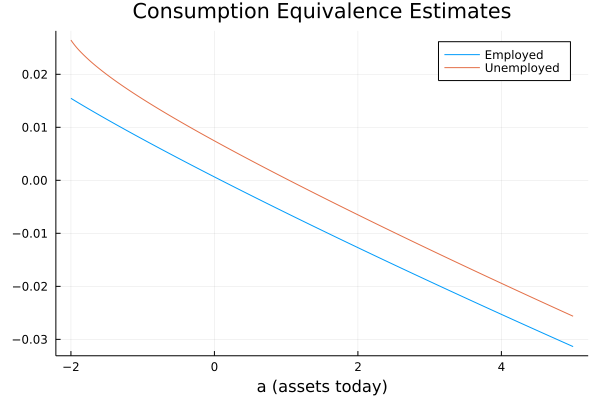
\includegraphics[width = 0.7\textwidth]{Lambda.png}
    \label{fig:lambda}
\end{figure}
\clearpage
\noindent\textbf{Incomplete Market Welfare and Welfare Costs: } Using the results from the computational exercise and the $\lambda(a,s)$ values described above, we can estimate the welfare of agents in an incomplete market:
\begin{align*}
    W_{INC} = \sum_{(a,s)\in A \times S} \mu(a, s) v(a, s) = -4.420 
\end{align*}
And the welfare gain of moving from an incomplete market to a complete market:
\begin{align*}
    W_{G} = \sum_{(a,s)\in A \times S} \lambda(a, s) \mu(a, s) = 0.0011
\end{align*}
Finally, the fraction of individuals who would like to move to the complete market is 
\begin{align*}
    \sum_{(a,s)\in A \times S} \one\{\lambda(a, s) \ge 0 \}(a, s) \mu(a, s) = 0.5224
\end{align*}
While the overall welfare gains are small (0.0011 is around 1/10 of 1 percent), over half of the population would like to move to the complete market. 


\end{document}

